% !TeX TS-program = pdflatex
% !BIB TS-program = biblatex

\documentclass[11pt,a4paper]{article}
\pdfoutput=1

% to be `\input` in subfolders,
% ... therefore the path should be relative to subfolders.

\usepackage{iftex}
\ifPDFTeX
\else
	\usepackage[UTF8
		,heading=false
		,scheme=plain % English Document
	]{ctex}
\fi
%\ctexset{autoindent=true}
\usepackage{indentfirst}

\input{../.modules/basics/macros.tex}
\input{../.modules/preamble_base.tex}
\input{../.modules/preamble_beamer.tex}
\input{../.modules/basics/biblatex.tex}


%Misc
	\usepackage{lilyglyphs}
	\newcommand{\indicator}{$\text{\clefG}$}
	\newcommand{\indicatorInline}{$\text{\clefGInline}$}

\newcommand{\legacyReference}{{
%	\clearpage\par
%	\quad\clearpage
	\def{\midquote}{\textbf{PAST WORK, AS TEMPLATE}}
	\newparagraph
}}

% Settings
\counterwithout{equation}{section}
\mathtoolsset{showonlyrefs=false}
%\DeclareTextFontCommand{\textbf}{\sffamily}

% Spacing
\geometry{footnotesep=2\baselineskip} % pre footnote split
\setlength{\parskip}{.5\baselineskip}
\renewcommand{\baselinestretch}{1.15}


%% List
%	\setlist*{
%		listparindent=\parindent
%		,labelindent=\parindent
%		,parsep=\parskip
%		,itemsep=1.2\parskip
%	}


\addtobeamertemplate{navigation symbols}{}{%
    \usebeamerfont{footline}%
%    \usebeamercolor[fg]{footline}%
    \hspace{1em}%
    \large\insertframenumber/\inserttotalframenumber
}

\makeatletter
\setbeamertemplate{headline}
{%
    \begin{beamercolorbox}[wd=\paperwidth,colsep=1.5pt]{upper separation line head}
    \end{beamercolorbox}
    \begin{beamercolorbox}[wd=\paperwidth,ht=2.5ex,dp=1.125ex,%
      leftskip=.3cm,rightskip=.3cm plus1fil]{title in head/foot}
      \usebeamerfont{title in head/foot}\insertshorttitle
    \end{beamercolorbox}
    \begin{beamercolorbox}[wd=\paperwidth,ht=2.5ex,dp=1.125ex,%
      leftskip=.3cm,rightskip=.3cm plus1fil]{section in head/foot}
      \usebeamerfont{section in head/foot}%
      \ifbeamer@tree@showhooks
        \setbox\beamer@tempbox=\hbox{\insertsectionhead}%
        \ifdim\wd\beamer@tempbox>1pt%
          \hskip2pt\raise1.9pt\hbox{\vrule width0.4pt height1.875ex\vrule width 5pt height0.4pt}%
          \hskip1pt%
        \fi%
      \else%  
        \hskip6pt%
      \fi%
      \insertsectionhead
    \end{beamercolorbox}
% Code for subsections removed here
}
\makeatother

\newcommand{\lui}[2]{\textcolor{red}{#1}\todo[color=yellow]{\scriptsize{L: #2}}}

%%%%%%%%%%%%%%%%%%%%%%%%%%%%%%%%%%%%%%%%%%%%%%




%%%%%%%%%%%%%%%%%%%%%%%%%%%%%%%%%%%%%%%%%%%%%%
%%%%%%%%%%%%%%%%%%%%%%%%%%%%%%%%%%%%%%%%%%%%%%
\title{Modular flow and holographic entanglement entropy in cutoff AdS} 
\author[a]{The EE $T\bar{T}$ Project}
%\author[a]{Luis Apolo,} 
%\author[a]{Pengxiang Hao,} 
%\author[a]{Wen-Xin Lai,}
%\author[a]{and Wei Song} 

\affiliation[a]{Yau Mathematical Sciences Center, Tsinghua University, Beijing 100084, China}
 

%  \emailAdd{apolo@mail.tsinghua.edu.cn, wsong2014@mail.tsinghua.edu.cn} 
 
\abstract{
	\begin{itemize}
	
	\item[] In Section 1,
	
	\item We follow the recipe from the swing surface proposal \cite{Apolo:2020bld,Apolo:2020qjm} to extend the boundary modular flow to the bulk, by matching symmetries of the bulk and the boundary.  This reproduces known results in e.g.~\cite{Lashkari:2016idm,Czech:2019vih,Apolo:2020qjm} \sidenote{[more citations needed]}. We first compute everything in Poincar\'e $\mrm{AdS}_3$ for simplicity. 
	
	\item We look at the flow at constant cutoff $z = z_c$, which has non-trivial $\pdd{z}$ component, which in turn leads to a violation of the $2\pi$ periodicity for $\xi$ along the horizon. This could be related to the violation of boosted strong subadditivity (boosted SSA) in \cite{Lewkowycz:2019xse}. 
	
	\item We then note that the periodicity can be restored by following the flow of $\xi$ starting from a codim-2 cutoff surface. This could be related to the \textit{restricted maximin} proposal of \cite{Marolf:2019bgj,Grado-White:2020wlb}. \sidenote{[With this cutoff the causal wedge again coincides with the entanglement wedge]}
	
	\item We try to obtain the entanglement entropy using the modular flow at the \mbox{codim-2} cutoff surface, using the \textit{effective inverse temperature $\beta(x)$} introduced in \cite{Wong:2013gua,Cardy:2016fqc}, which relates the entanglement entropy to some thermal entropy. \sidenote{[relation with partial entanglement entropy?]}
	
	\item \sidenote{We should look at the boosted interval.}
	
	\item[] In Section 2,
	
	\item We map the the modular flow in the Poincar\'e $\mrm{AdS}_3$ vacuum to the BTZ background, and compute the entanglement entropy as gravitational charge. 
	
	\item We then consider constant $r$ cutoff in the Schwarzschild coordinates, which corresponds to the proposal of \cite{McGough:2016lol}. This gives a finite temperature generalization of the result of \cite{Lewkowycz:2019xse}. 
	
	\end{itemize}
}
%%%%%%%%%%%%%%%%%%%%%%%%%%%%%%%%%%%%%%%%%%%%%%
%%%%%%%%%%%%%%%%%%%%%%%%%%%%%%%%%%%%%%%%%%%%%%





%%%%%%%%%%%%%%%%%%%%%%%%%%%%%%%%%%%%%%%%%%%%%%
%%%%%%%%%%%%%%%%%%%%%%%%%%%%%%%%%%%%%%%%%%%%%%
%%%%%%%%%%%%%%%%%%%%%%%%%%%%%%%%%%%%%%%%%%%%%%
\begin{document}
\maketitle
%\flushbottom
%%%%%%%%%%%%%%%%%%%%%%%%%%%%%%%%%%%%%%%%%%%%%%
%%%%%%%%%%%%%%%%%%%%%%%%%%%%%%%%%%%%%%%%%%%%%%
%%%%%%%%%%%%%%%%%%%%%%%%%%%%%%%%%%%%%%%%%%%%%%

\setlength{\parskip}{.5\baselineskip}

\addtocounter{section}{-1}
\section{Conventions}
	We try to follow the conventions of the TsT paper \textcite{Apolo:2019zai}. 
	\begin{itemize}
	\item Lightcone coordinates: $u,v = x\pm t$, similar to \cite{Apolo:2019zai}. This convention has the following features:
	
		\begin{itemize}
		\item The constant $t$ slice is given by $u = v$;
		\item It preserves the orientation as we go from $(t,x)$ to $(u,v)$. Note that the ordering of coordinates matters here.
		\end{itemize}
	
	\item Poincar\'e $\mrm{AdS}_3$ coordinates: $
			X^I \sim (x^\mu,z) \sim (t,x,z) \sim (u,v,z)
		$, metric: 
	\begin{equation}
		\dd{s}^2
		= \frac{+\dd{u} \dd{v} + \dd{z}^2}{z^2}
	\end{equation}
	Note the \mquote{+} before $\dd{u} \dd{v}$. 
	
	\item The $T\bar{T}$ deformation is parametrized by the deformation parameter $\mu$ with mass dimension $(-2)$, defined in \cite{Apolo:2019zai}; sometimes it is more convenient to use the dimensionless \textit{worldsheet} deformation parameter $\lambda = \mu/\ell_s^2$, where $\ell_s$ is the string length. See \cite{Apolo:2019zai} section 2.3 and its (2.43). 
	
	\item Coordinate length of the boundary interval $\mcal{A}$ at the asymptotic infinity is denoted as $L_\infty$; the coordinate length at finite cutoff is denoted as $L$. For an interval lying on the constant time slice $t = 0$ in the Poincar\'e patch, we have $L = \Delta x$; for a boosted interval, we have $
		L = \eta_{\mu\nu}\, \Delta x^\mu\, \Delta x^\nu
	$. 
	\end{itemize}
	
	
\pagebreak

\section{Introduction}

\section{Boundary story }
\subsection{boundary modular flow}
\subsection{local temperature trick}
\subsection{}


\section{Bulk story}
\subsection{Bulk modular flow}
\subsection{gravitational charges}






\section{Zero temperature: modular flow in the Poincar\'e patch}
	
\subsection{Review of the general recipe}
	A boundary interval $\mcal{A}$ defines a denisty matrix:
	\begin{equation}
		\rho_\mcal{A}
		= \tr_{\bar{\mcal{A}}} \rho
		= e^{-\mcal{H}_\mcal{A}}
	\end{equation}
	where $\bar{\mcal{A}}$ is the complement of $\mcal{A}$ and $\mcal{H}_\mcal{A}$ is the corresponding modular Hamiltonian. $\mcal{H}_\mcal{A}$ is generically nonlocal, but in a highly symmetric background (e.g.~AdS vacuum) it might be geometrically realized and corresponds to a symmetry of the underlying quantum field theory. This is the modular flow $\xi$. 
	
	In such case there is a generalized Rindler transformation $f$ that maps the casual domain $\mcal{D}$ to a patch $\{(\tau,\tilde{x})\}$ in some noncompact generalized Rindler spacetime, with $\pdd{\tau}$ an isometry of the spacetime. Then we have:
	\begin{equation}
		\xi = 2\pi \pdd{\tau}
		= 2\pi \sum_i a^i H_i,
	\quad
		\tau \sim \tau + 2\pi i
		= \tau + i\beta_\tau,
	\quad
		\beta_\tau = 2\pi
	\end{equation}
	Here $H_i$ are the symmetry generators. The causal domain of dependence $\mcal{D}$ is mapped to some thermal state with normalized inverse temperature $\beta_\tau = 2\pi$. Here we choose to absorb such $2\pi$ into the definition of $\xi$, so the Euclidean periodicity w.r.t.~$\xi$ is simply $\beta_\xi = 1$, which means the surface gravity along the horizon is given by:
	\begin{equation}
		\kappa_\xi = \frac{2\pi}{\beta_\xi} = 2\pi,
	\quad
		\beta_\xi = 1
	\end{equation}

\pagebreak

\subsection{Modular flow for Poincar\'e $\mrm{AdS}_3/\mrm{CFT}_2$}

\textbf{Summary:} We follow the recipe from the swing surface proposal \cite{Apolo:2020bld,Apolo:2020qjm} to extend the boundary modular flow to the bulk, by matching symmetries of the bulk and the boundary. This reproduce known results such as \cite{Lashkari:2016idm,Czech:2019vih,Apolo:2020qjm} [more citations needed].

\noindent\textbf{Mathematica:} \texttt{modFlowPoincare.nb}

\subsubsection{Matching bulk and boundary symmetries}
	In Poincar\'e $\mrm{AdS}_3/\mrm{CFT}_2$, the $H_i$'s are given by $L_n,\tilde{L}_n$ with $n=0,\pm 1$. At $z\to 0$ we recover the usual global $\mfrak{sl}(2,\mbb{R})$ generators:
	\begin{equation}
		z\to 0,
	\quad
		      L_n \to -u^{n+1} \pdd{u},\quad
		\tilde{L}_n \to -v^{n+1} \pdd{v},\quad
	n = 0,\pm 1
	\end{equation}
	
	To extend it to the bulk, think of the corresponding bulk isometries: translations, rotations, dilations and special conformal transformations:
	\begin{equation}
	\begin{aligned}
		P_\mu
		&= \pdd{\mu},\\
		m_{uv}
		&= x_\mu \pdd{\nu} - x_\nu \pdd{\mu}
		= u\pdd{u} - v\pdd{v},\\
		\Delta
		&= X^I \pdd{I}
		= u\pdd{u} + v\pdd{v} + z\pdd{z},\\
		K_\mu
		&= (z^2 + uv)\,\pdd{\mu}
			- 2\eta_{\mu\nu} x^\nu \Delta,
	\end{aligned}
	\end{equation}
	\begin{equation}
		K_u = (z^2 + uv)\,\pdd{u} - v \Delta,
	\quad
		K_v = (z^2 + uv)\,\pdd{v} - u \Delta
	\end{equation}
	By requiring that a linear combination of these generators reduce to the boundary $L_n$'s, one can uniquely extend the $L_n,\tilde{L}_n$'s into the bulk. The result for $L_n$'s is listed below; for $\tilde{L}_n$ one need only exchange all $u\leftrightarrow v$.
	\begin{equation}
		L_{-1} = -\pdd{u},
	\quad
		L_0 = -u\,\pdd{u} - \frac{z}{2}\,\pdd{z},
	\quad
		L_1 = -u^2\pdd{u} + z^2 \pdd{v}
			- uz\,\pdd{z}
	\end{equation}

\subsubsection{RT surface and the modular flow}

\textbf{Derivation of RT surface:} \\
 \url{https://bryango.github.io/resources/archive/HW-Gravity/gravity1.pdf}. 

	The RT surface (spacelike geodesic of Poincar\'e AdS with both ends attached to the boundary) is parametrized in terms of its end points $(t,x)_\pm$; it's the intersection of a AdS ``sphere'' (hyperboloid) and a plane through its center:
	\begin{equation}
	\begin{aligned}
	\text{``sphere'':} &&&\mathsmaller{
		z^2
		+ \pqty{x - \frac{x_+ + x_-}{2}}^{\!\!2}
		- \pqty{t - \frac{t_+ + t_-}{2}}^{\!\!2}
		= \pqty{\frac{L_\infty}{2}}^{\!\!2}
		= \pqty{\frac{x_+ - x_-}{2}}^{\!\!2}
		- \pqty{\frac{t_+ - t_-}{2}}^{\!\!2}
	},\\
	&&& \text{i.e.}\ \,
		L^2
		= \pqty{x_+ - x_-}^2
			- \pqty{t_+ - t_-}^2
		= (u_+ - u_-)(v_+ - v_-),
	\\[1.5ex]
	\text{plane:} &&&
		\frac{x - \frac{1}{2} (x_+ + x_-)}{x_+ - x_-}
		= \frac{t - \frac{1}{2} (t_+ + t_-)}{t_+ - t_-}
	\end{aligned}
	\end{equation}
	Alternatively, it can be more compactly rewritten with $x^\mu \sim (t,x)$ or $(u,v)$; mind the various $\pm$ signs in the expressions: 
	\begin{equation}
	\begin{aligned}
		0 &= z^2
			+ \eta_{\mu\nu} (x - x_+)^\mu (x - x_-)^\nu \\
		& = z^2
			+ (x - x_+)(x - x_-)
			- (t - t_+)(t - t_-) \\
		&= z^2 + \frac{
				(u - u_+)(v - v_-)
				+ (v - v_+)(u - u_-)
			}{2}
	\end{aligned}
	\end{equation}
	
	The bulk modular generator vanishes along the RT surface, i.e.~the RT surface is the fixed point of the modular flow; with this condition we can fix the coefficients of the modular generator, up to an overall coefficient\footnote{
		One can compare this with similar results in the literature such as \cite{Lashkari:2016idm,Czech:2019vih,Apolo:2020qjm}. 
	}:
	\begin{equation}
		\xi = 2\pi \sum_{n=0,\pm 1} \pqty{
				s_n L_n - \tilde{s}_n \tilde{L}_n
			},
	\end{equation}
	\begin{equation}
		s_{-1} = \frac{u_+ u_-}{u_+ - u_-},\quad
		s_0 = - \frac{u_+ + u_-}{u_+ - u_-},\quad
		s_{+1} = \frac{1}{u_+ - u_-}
	\end{equation}
	One need only exchange all $u\leftrightarrow v$ to obtain $\tilde{s}_n$. The overall coefficient of $\xi$ (in this case, $2\pi$) is fixed by normalizing the temperature of the horizon, namely we demand that the surface gravity is $2\pi$ along the RT surface:
	\begin{equation}
		\beta_\xi = \frac{2\pi}{\kappa_\xi} = 1,
	\quad
		\kappa_\xi^2
		= (2\pi)^2
		= -\frac{1}{2}\,
			(\nabla_{\mu} \xi_{\nu})
			(\nabla^{\mu} \xi^{\nu})
	\end{equation}
	
	\begin{figure}[!ht]
%	\vspace{-1.5ex}
	\centering
	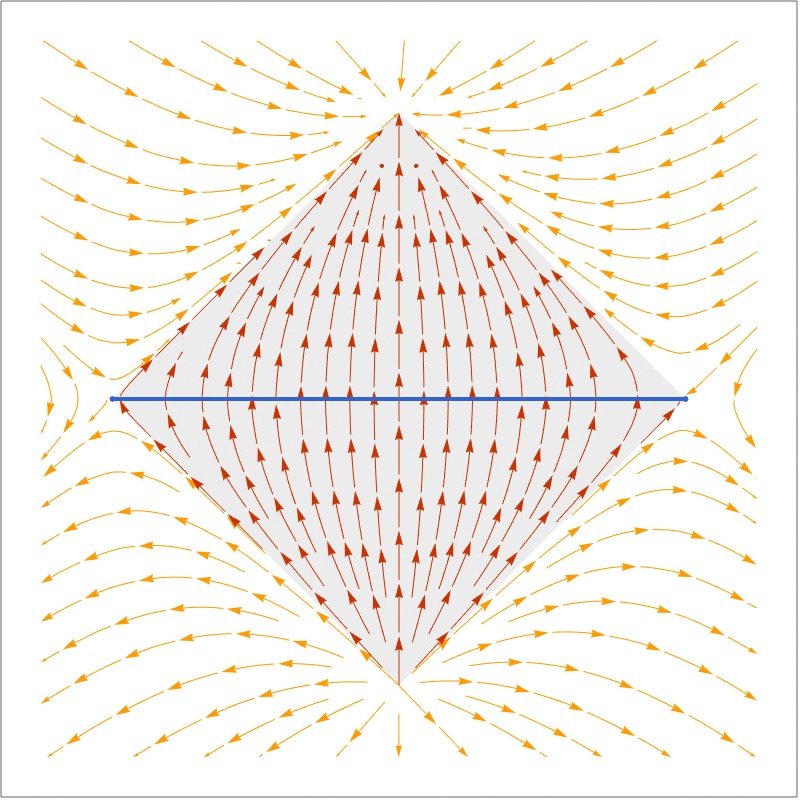
\includegraphics[width=.4\linewidth]{img/modFlowLorentzian.png}
	\hspace{2em}
	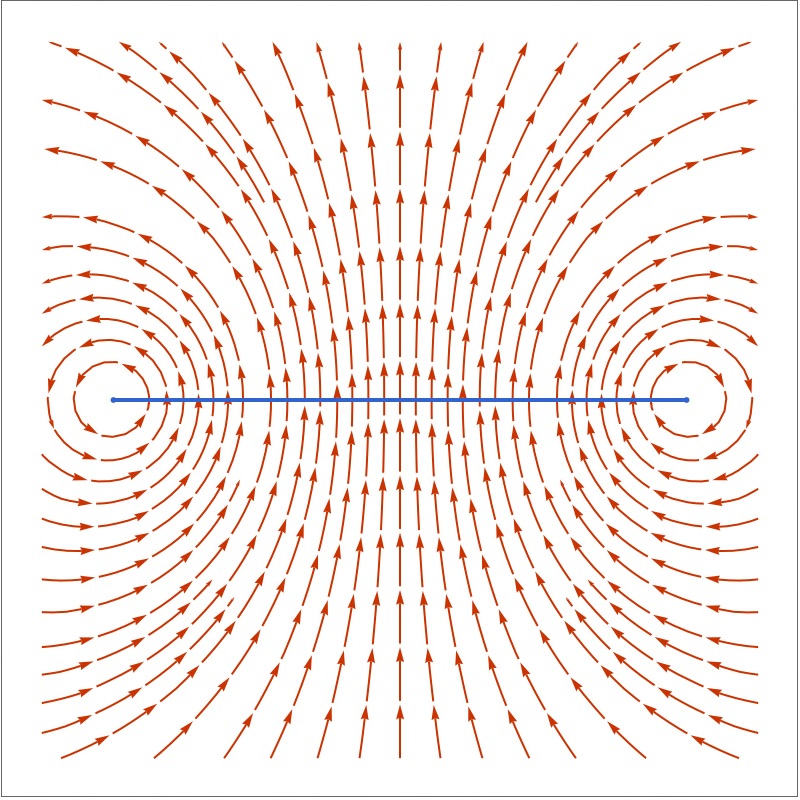
\includegraphics[width=.4\linewidth]{img/modFlowEuclidean.png}
%	\vspace{-2ex}
	\caption{Modular flow at the boundary, for an interval lying on a constant $t = 0$ slice, in Lorentzian and Euclidean signature}
	\end{figure}
	
\pagebreak[4]
	
	We now restrict to an interval centered at the origin: $
		u_\pm v_\pm
		= x^2_\pm - t^2_\pm
		= (\frac{L_\infty}{2})^2
	$, where $x_\pm = -x_\mp$, and same for $t_\pm, u_\pm, v_\pm$. 
	We then introduce the \textit{rapidity} $\theta$ to nicely parametrized the boosted interval; for a constant time slice, we have $\theta = 0$. For a general boosted interval, we have:
	\begin{equation}
		x_\pm = \pm \frac{L_\infty}{2} \cosh \theta,
	\quad
		t_\pm = \pm \frac{L_\infty}{2} \sinh \theta,
	\end{equation}
	For now the coordinates $u_\pm, v_\pm, x_\pm, t_\pm$ and the coordinate length $L_\infty$ are all specified at $z\to 0$, i.e.~at the \textbf{asymptotic boundary}. Note that the RT surface lies on the plane $
		t_\pm / x_\pm = \tanh \theta
	$, namely $\theta$ is constant along the RT surface. 
	We have:
	\begin{gather}
	\begin{aligned}
		\xi &= \frac{2\pi}{L_\infty} \bigg\{
			\pqty\Big{
				\pqty{
					(\tfrac{L_\infty}{2})^2 - z^2
					- (t^2 + x^2)
				} \cosh\theta
				+ 2tx \sinh\theta
			} \,\pdd{t}
		\\ &\qquad\qquad 
			+ \pqty\Big{
				\pqty{
					(\tfrac{L_\infty}{2})^2 - z^2
					+ (t^2 + x^2)
				} \sinh\theta
				- 2tx \cosh\theta
			} \,\pdd{x}
		\\ &\qquad\qquad 
			+ \pqty\big{
				x\sinh\theta
				- t\cosh\theta
			} \,2z\pdd{z}
		\bigg\}
	\end{aligned}
	\end{gather}
	
	We note that the $\pdd{z}$ term vanishes in the following two cases:
	\begin{itemize}[noitemsep,topsep=0pt]
	\item as $z\to 0$, i.e.~near the asymptotic boundary;
	\item within the whole plane: $
			x\sinh\theta
			= t\cosh\theta
		$ where the RT surface lies. 
	\end{itemize}
	
\FloatBarrier
\pagebreak
\subsection{Cutoff $\mrm{AdS}_3$ and the loss of $2\pi$ periodicity}

\textbf{Summary:} We look at the flow at constant cutoff $z = z_c$, which has non-trivial $\pdd{z}$ component, which in turn leads to a violation of the $2\pi$ periodicity for $\xi$ along the horizon.
	
	Now we'd like to study $\xi$ not at the asymptotic boundary, but at some \textbf{constant finite cutoff} $z = z_c$. 
	Note that is the size (coordinate length) of the interval at the {asymptotic boundary}; the coordinate length of the \textbf{cutoff interval $L$}, on the other hand, is given by:
	\begin{equation}
		\pqty{\frac{L}{2}}^{\!\!2}
		= \pqty{\frac{L_\infty}{2}}^{\!\!2} - z_c^2,
	\quad
		x_\pm^c
		= \pm \frac{L}{2}
	\label{eq:length_relations}
	\end{equation}
	
	We then consider $\xi$ evaluated at the {constant finite cutoff} $z = z_c$,
	\begin{equation}
	\begin{aligned}
		\xi|_{z=z_c}
		= \frac{2\pi}{
				L\sqrt{1 + (2z_c/L)^2}
			}
		& \bigg\{
			\pqty\Big{
				\pqty{
					(\tfrac{L}{2})^2
					- (t^2 + x^2)
				} \cosh\theta
				+ 2tx \sinh\theta
			} \,\pdd{t}
		\\[-.5ex] &\quad 
			+ \pqty\Big{
				\pqty{
					(\tfrac{L}{2})^2
					+ (t^2 + x^2)
				} \sinh\theta
				- 2tx \cosh\theta
			} \,\pdd{x}
		\\ &\quad 
			+ \pqty\big{
				x\sinh\theta
				- t\cosh\theta
			} \,2z_c\pdd{z}
		\bigg\}
	\end{aligned}
	\end{equation}
	Note that the $\pdd{z}$ component is generally non-zero, i.e.~$\xi|_{z=z_c}$ is not entirely contained in the $z = z_c$ plane. 
	We observe the factor $
		\sqrt{1 + (2z_c/L)^2}
	$ which is featured prominently in the $T\bar{T}$ deformed $C(L)$ function, given in \cite{Lewkowycz:2019xse}:
	\begin{equation}
		C(L) = L\,\pdd{L} S(L)
		= \frac{c}{3} 
			\frac{1}{
				\sqrt{1 + (2z_c/L)^2}
			}
	\end{equation}
	
	This seems nice and all but there is a subtlety for finite cutoff $z = z_c$. 
	In the bulk the constant surface gravity $
		\xi^\nu \cdv{\nu} \xi^\mu
		= \kappa_\xi \xi^\mu
		= 2\pi \xi^\mu
	$ guarantees that after Wick rotation, the Euclidean periodicity around the horizon is normalized to $\beta = 1$. However, if we restrict to the field theory living at constant cutoff $z = z_c$, which corresponds to a $T\bar{T}$ deformed theory \cite{McGough:2016lol,Lewkowycz:2019xse} \sidenote{[more citations needed]}, since it has no knowledge of the $\pdd{z}$ component of $\xi$, we should reduce it to a modular flow within the $z = z_c$ plane by, e.g.~projecting the $z$ component out, which leaves us:
	\begin{equation}
	\begin{aligned}
		\xi^{\mrm{FT}}_c
		\equiv \proj{\sslash} \xi|_{z_c}
		= \frac{2\pi}{
				\sqrt{1 + (2z_c/L)^2}
			}
		& \bigg\{
			\pqty\Big{
				\pqty{
					(\tfrac{L}{2})^2
					- (t^2 + x^2)
				} \cosh\theta
				+ 2tx \sinh\theta
			} \,\pdd{t}
		\\[-2ex] &\quad 
			+ \pqty\Big{
				\pqty{
					(\tfrac{L}{2})^2
					+ (t^2 + x^2)
				} \sinh\theta
				- 2tx \cosh\theta
			} \,\pdd{x}
		\bigg\}
	\end{aligned}
	\end{equation}
	Which no longer has normalized $\beta$ if $z_c \ne 0$. In fact, compared to the $z_c \to 0$ situation which \textit{does} have $\beta = 1$, $\xi^{\mrm{FT}}_c$ is rescaled by a factor of $
		\frac{L}{L_\infty}
		= 1/\sqrt{1 + (2z_c/L)^2}
	$, which means that:
	\begin{equation}
		\beta^{\mrm{FT}}_c
		= \sqrt{1 + (2z_c/L)^2}
		\sim 1 + 2z_c^2 / L^2
	\end{equation}
	
	\begin{figure}[!ht]
	\vspace{-1.5ex}
	\centering
	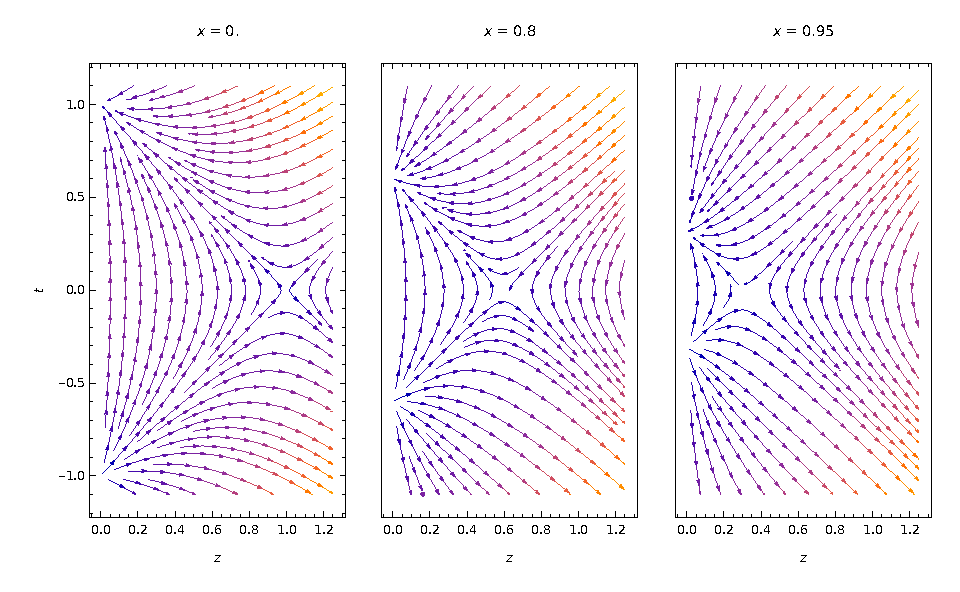
\includegraphics[width=.8\linewidth]{img/modFlowXsection.pdf}
	\hspace{2em}
	\vspace{-2ex}
	\caption{Modular flow at constant $x$ slices}
	\end{figure}
	
\pagebreak[3]
	
	How should we understand this?
	\begin{itemize}
	\item The $T\bar{T}$ deformation might somehow correspond to a variation of temperature at the cutoff; instead of $\rho = e^{-\mcal{H}}$, we now have:
	\begin{equation}
		\rho = e^{-\beta\mcal{H}},
	\quad \beta \sim 1 + \frac{1}{L^2} \order{\mu}
	\end{equation}
	Where $\mu$ is the deformation parameter (see \cite{Apolo:2019zai} for the convention we follow). \sidenote{This might also be related to the \textit{local entanglement temperature} defined in later sections.}
%	Q: how do we make this precise?
	
	\item The non-local nature of $T\bar{T}$ deformation creates some $\order{z_c}$ ``fuzziness'' in the cutoff theory at $z = z_c$; $\beta \sim 1$ holds only up to some coarse-graining of points. 
%	Q: again, how do we make this precise?
	
	\item Maybe we shouldn't project out the $\pdd{z}$ component of $\xi$, but instead \textit{define} the cutoff by following the flow of $\xi = 2\pi\pdd{\tau}$; in this way the periodicity is preserved by construction: $\beta_\xi = 1$. We will discuss this in the next section. 
	\end{itemize}
	
\pagebreak
\subsection{Restoring the $2\pi$ periodicity by following the flow}
	
\textbf{Summary:} We note that the periodicity can be restored by following the flow of $\xi$ starting from a codim-2 cutoff surface. This is related to the proposal of \cite{Grado-White:2020wlb}. 
	
	Instead of projecting out the $\pdd{z}$ component of $\xi$, we could \textit{define} the evolution of the cutoff interval by following the flow of $\xi = 2\pi\pdd{\tau}$ starting from the RT surface at $z = z_c$. Now there is no longer a projection of $\xi$; we are always following it along the boundary, so the periodicity is preserved: $\beta = 1$. 
	
	But now this is no longer a \textit{constant} cutoff away from $z = z_c$. In particular, the forward and backward evolved interval will approach the upper and lower endpoints of the diamond at $z \to 0$. Q: will it be compatible with \textcite{McGough:2016lol}? 
	
	\sidenote{\textbf{On the other hand, this seems highly related to the restricted maximin proposal of \cite{Marolf:2019bgj,Grado-White:2020wlb} [comments needed],}} which discusses the violation of boosted strong subadditivity (SSA) due to the constant finite cutoff observed in \cite{Lewkowycz:2019xse}, and offers a similar resolution of using a codim-2 cutoff surface instead of the usual codim-1 cutoff. Namely, the cutoff is given by $
		z = z_c, t = 0
	$, instead of just $z = z_c$. 
	
	\begin{figure}[!ht]
	\centering
%	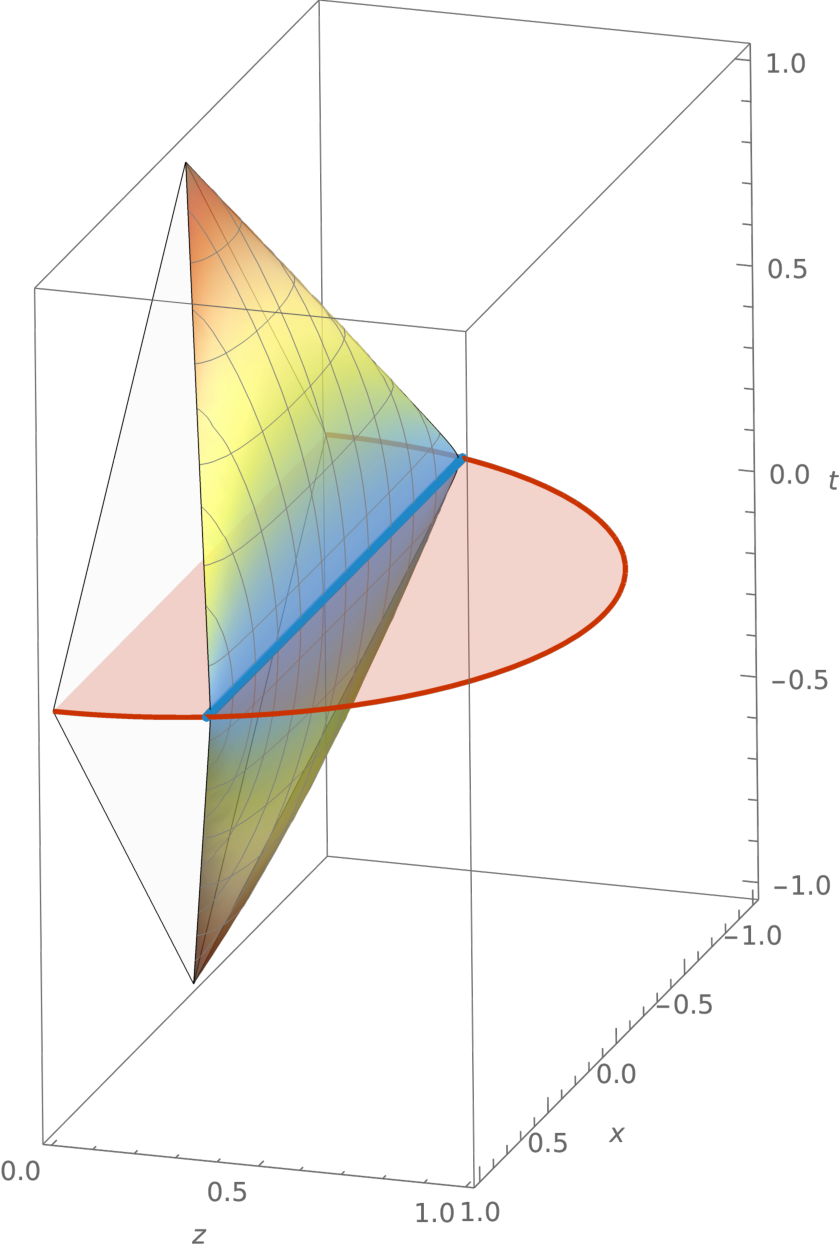
\includegraphics[width=.35\linewidth]{img/modFlowCutoff.pdf}
	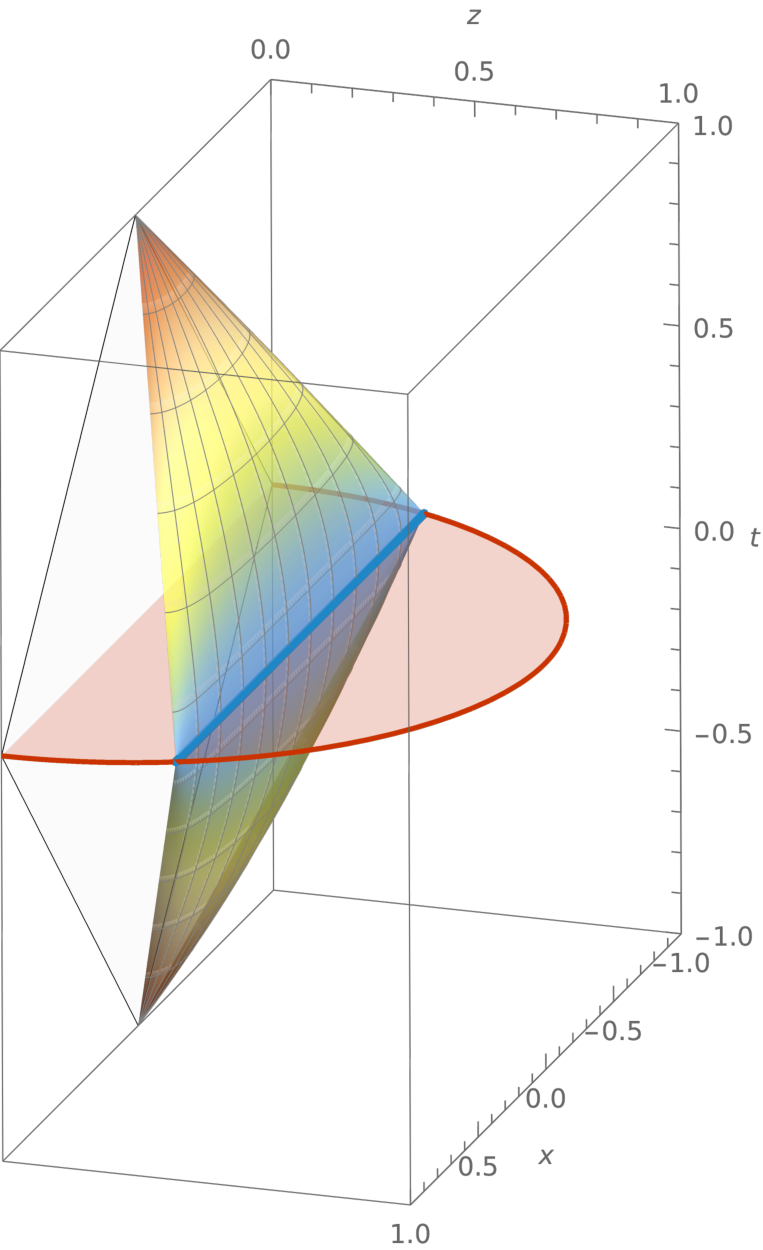
\includegraphics[width=.35\linewidth]{img/modFlowAnalytic.pdf}
%	\hspace{2em}
%	\vspace{-2ex}
	\caption{Integral surface of the modular flow starting from $t = 0,\ z = z_c$. Here we've chosen $\frac{L_\infty}{2} = 1$ while $z_c = 0.4$.}
	\end{figure}
	
\pagebreak
	
	For an interval lying on a constant time slice $t_\pm = 0$, i.e.~$\theta = 0$, we can actually solve the flow of $\xi$ without much difficulty.
	Consider the flow starting from $(t,x,z) = (0,x_c,z_c)$, we note that $
		\dd{x}/\dd{z}
		= {\dv{x}{\lambda}}/{\dv{z}{\lambda}}
		= {x}/{z}
	$, which implies that ${x}/{x_c} = {z}/{z_c}$ along the flow lines. Intuitively, the flow when restricted in $x$-$z$ plane points towards / away froms $x = z = 0$, which is the upper / lower tip of the entanglement wedge. 
	
	We can further replace the flow parameter $\lambda$ with time coordinate $t$ by considering $
		\dd{z}/\dd{t}
		= {\dv{z}{\lambda}}/{\dv{t}{\lambda}}
	$, which leads to the following equations:
	\begin{equation}
		\dv{z}{t}
		= \frac{2tz}{\alpha z^2 + t^2 - (L_\infty/2)^2},
	\quad
		\alpha = 1 + \frac{x_c^2}{z_c^2},
	\quad
		\frac{x}{x_c} = \frac{z}{z_c}
	\end{equation}
	The solution is then given by:
	\begin{equation}
		z = z(t;x_c,z_c)
		= \frac{
				(L_\infty/2)^2 + \alpha z_c^2
				- \sqrt{
					\pqty\big{(L_\infty/2)^2 - \alpha z_c^2}^2
					+ 4t^2 \alpha z_c^2
				}
			}{2\alpha z_c}
	\end{equation}
	
%	
	
	To gain more understanding of the modular flow of the cutoff theory, we can look at the \textit{CHM map} \cite{Casini:2011kv} to the Rindler coordinates. In the Poincar\'e $\mrm{AdS}_3$ case this is explicitly given in Appendix B of \cite{Song:2016gtd}; the entanglement wedge in Poincar\'e $(t,x,z)$ is mapped to the planar BTZ $(u,v,\rho)$:
	\begin{equation}
	\begin{aligned}
		t &= \frac{L_\infty}{2} \frac{
				\pqty{\rho - T_u T_v}
				\,\sinh\,(T_u u - T_v v)
			}{
				\sqrt{\rho^2 - T_u^2 T_v^2}
					\,\cosh\,(T_u u + T_v v)
				+ \pqty{\rho - T_u T_v}
					\,\cosh\,(T_u u - T_v v)
			},
	\\
		x &= \frac{L_\infty}{2} \frac{
				\sqrt{\rho^2 - T_u^2 T_v^2}
				\,\sinh\,(T_u u + T_v v)
			}{
				\sqrt{\rho^2 - T_u^2 T_v^2}
					\,\cosh\,(T_u u + T_v v)
				+ \pqty{\rho - T_u T_v}
					\,\cosh\,(T_u u - T_v v)
			},
	\\
		z &= \frac{L_\infty}{2} \frac{
				\sqrt{2T_u T_v}
				\sqrt{\rho - T_u T_v}
			}{
				\sqrt{\rho^2 - T_u^2 T_v^2}
					\,\cosh\,(T_u u + T_v v)
				+ \pqty{\rho - T_u T_v}
					\,\cosh\,(T_u u - T_v v)
			},
	\end{aligned}
	\label{eq:poincare2btz}
	\end{equation}
	\begin{equation}
		\dd{s}^2
		= \frac{\dd{\rho}^2}{4\,(\rho^2 - T_u^2 T_v^2)}
			+ T_u^2 \dd{u}^2
			+ T_v^2 \dd{v}^2
			+ 2\rho \dd{u} \dd{v},
	\end{equation}
	This is a BTZ \textit{black string} with \textit{non-compact} $\phi$ direction. 
	One can check that the $(u,v,\rho)$ coordinates indeed cover the $L_\infty$-sized entanglement wedge specified by $\xi$. 
	Here we've reused the variable names $(u,v)$ for the planar BTZ coordinates, and we've tweaked the expressions in \cite{Song:2016gtd} to be more symmetric in $(u,v)$. 
	
	\noindent\sidenote{\textbf{TO CHECK:}} At the boundary this reduces to the result of \textcite{Casini:2011kv}, which is used by \textcite{Lewkowycz:2019xse}. Also see the note \texttt{EETTbar.pdf}. 
	
	We note that $T_{u,v}$ is \textit{not quite} the physical Hawking temperature of the spacetime; the physical temperature is given by (see e.g.~\cite{Compere:2018aar}):
	\begin{equation}
		T_\tau = \frac{\kappa_\tau}{2\pi}
		= \frac{1}{\pi}\,
			\frac{2}{T_u^{-1} + T_v^{-1}},
	\quad
		\tau = \frac{u - v}{2}
	\end{equation}
	For $T_u = T_v = T$, we have $T_\tau = \frac{T}{\pi}$, i.e.~the Hawking temperature differs from $T_u = T_v = T$ by a factor of $\frac{1}{\pi}$. In this case, the temperature can also be found easily by Euclidean expansion around the horizon $\rho = T_u T_v \cosh r$,
	\begin{gather}
		\dd{s}^2|_{\rho,\tau}
		\sim \frac{1}{4} \dd{r}^2
			+ 2T^2 \pqty{\cosh r - 1}
				\dd{\tau}^2
		\sim \frac{1}{4}\,\pqty{
				\dd{r}^2
				+ (2T)^2\,r^2 \dd{\tau}^2
			},
	\\[1ex]
		2T\beta_\tau = 2\pi,
	\quad
		T_\tau = \frac{1}{\beta_\tau} = \frac{T}{\pi}
	\end{gather}
	
	To achieve our normalization convention $\xi = 2\pi \pdd{\tau}$ as before, we simply set:
	\begin{equation}
		\beta_\tau = 2\pi,
	\quad
		T_u = T_v = T = \frac{1}{2}
	\end{equation}
	We can then verify using the coordinate transformation \eqref{eq:poincare2btz} that the modular generator in these coordinates is indeed what we are expecting:
	\begin{equation}
		\xi
		= 2\pi\,(\pdd{u} - \pdd{v})
		= 2\pi\pdd{\tau}
	\end{equation}
	
	With these planar BTZ coordinates, the flow of $\xi = 2\pi\pdd{\tau}$ is almost trivial; we need only identify the initial conditions, which is given by $z = z_c$ and $t = 0$ in Poincar\'e coordinates. The integral surface is thus given by:
	\begin{equation}
		z_c = \frac{L_\infty}{2} \frac{
				\sqrt{2}\,T
				\sqrt{\rho - T^2}
			}{
				\sqrt{\rho^2 - T^4}
					\,\cosh\,(2T\phi)
				+ \pqty{\rho - T^2}
			},
	\quad
		T_u = T_v = T = \frac{1}{2}
	\end{equation}
	
	\begin{figure}[!ht]
	\centering
	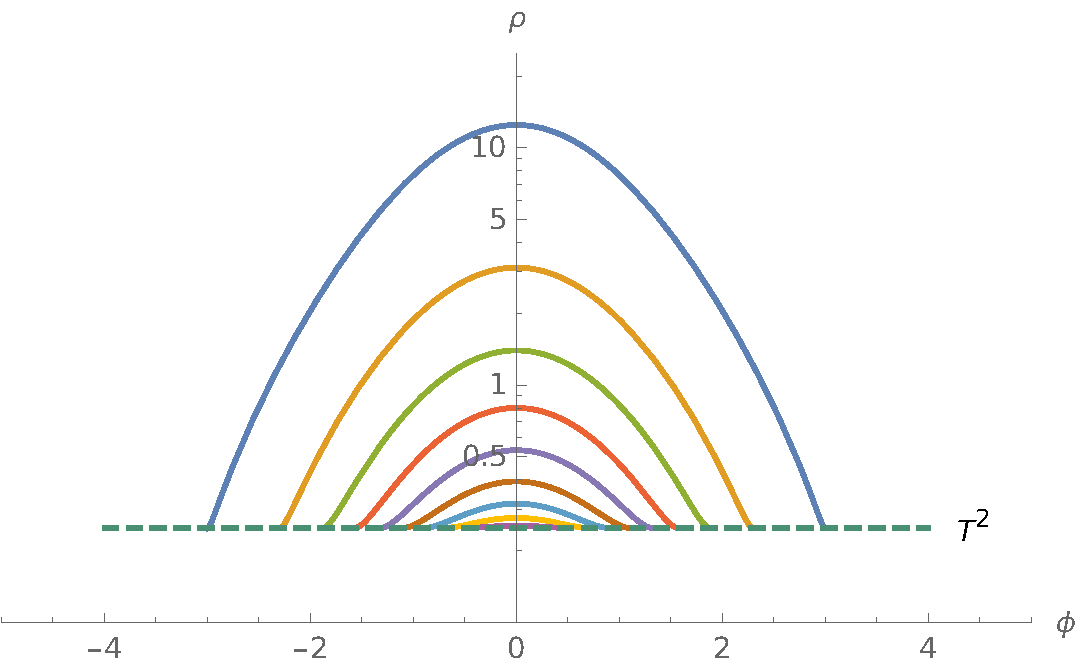
\includegraphics[width=.6\linewidth]{img/modFlowCutoff2BTZ.pdf}
%	\hspace{2em}
%	\vspace{-2ex}
	\caption[Integral surface of the modular flow when mapped to the planar BTZ coordinates]{%
		Integral surface of the modular flow when mapped to the planar BTZ coordinates. Note that the $\rho$ axis is logarithmic. 
		
		The flow starts from $t = 0,\ z = z_c$, and here we've chosen $\frac{L_\infty}{2} = 1$ while $z_c = 0.1,\,0.2,\,\cdots,\,0.9$. 
		Note that the asymptotic boundary $z\to 0$ corresponds to $\rho \to \infty$. 
		Also we've taken $T_u = T_v = T = \frac{1}{2}$ as discussed before, and the horizon is at $\rho = T_u T_v = T^2$; this is the image of the RT surface under the CHM map.
	}
	\end{figure}
	
\pagebreak[3]
	
	This is a surface in the planar BTZ coordinates that parallels $\pdd{\tau}$ and intersects the horizon. The horizon length, which is ``cut off'' by this surface, gives the finite entropy of the cutoff interval.
	With some basic algebraic manipulation, this can be solved in terms of $\rho(\phi)$:
	\begin{equation}
		\rho(\phi;z_c)
		= T^2 \pqty{
			1 + \frac{1}{2} \pqty{
				\frac{
					\cosh\,(2T\phi) \sqrt{
						1 - (\frac{2z_c}{L_\infty})^2 \sinh^2 (2T\phi)
					} - 1
				}{z_c\sinh^2 (2T\phi)}
			}^{\!\!\!\!2\ }
		},\quad
		T = \frac{1}{2}
	\end{equation}
	
\textit{
	We note that there is also a mysterious square root structure here: $\mathsmaller{
		\sqrt{
			1 - (\frac{2z_c}{L_\infty})^2 \sinh^2 (2T\phi)
		}
	}$, which resembles the familiar $
		\sqrt{1 + (\frac{2z_c}{L})^2}
	$ but has a minus sign, and the $\frac{2z_c}{L}$ factor is weighted by $\sinh\,(2T\phi)$. 
}	
	
	\sidenote{One oddity of this prescription is that the codim-1 cutoff geometry depends on the choice of the interval $\mcal{A}$}. This seems to suggest that there is no canonical way to embed the entire time-evolved deformed field theory into the bulk. The best we can do is to embed the causal diamonds $\mcal{D}(\mcal{A}) \cup \mcal{D}(\bar{\mcal{A}})$, given an interval $\mcal{A}$ and its complement $\bar{\mcal{A}}$. This is the price we have to pay for SSA to hold. 
	
	Maybe we should not expect that the entire time-evolved deformed theory can be embedded into the bulk. \sidenote{We could look at the proof of $T\bar{T}$ duality and check if this is really implied. It is quite possible that we only need to embed the boundary theory at a specific time slice, and the trace flow arguments will go through.}
	
	
\pagebreak
\subsection{Modular flow for the cutoff field theory}
\textbf{Summary:} We try to obtain the entanglement entropy using the modular flow at the \mbox{codim-2} cutoff surface, using the \textit{effective inverse temperature $\beta(x)$} introduced in \cite{Cardy:2016fqc}, which relates the entanglement entropy to some thermal entropy. 
	
	From the field theory's perspective, the above calculations seem to suggest that the modular flow $\xi$ of [[ an $L$-sized interval in the cutoff theory ]] is given by the modular flow $\xi = \xi(L_\infty)$ of [[ a CFT for an $L_\infty$ interval ]]. 
	
	We note that there is a trick to read out the entanglement entropy from the modular flow: it is possible to define a \textit{local entanglement temperature}, and then use it to read the entanglement entropy from the modular flow generator \cite{Cardy:2016fqc}. The result is obtained by comparing with the Hamiltonian of a thermal field theory, where we have:
	\begin{equation}
	\mcal{H}=\int \beta\,T_{00}\,dx,\quad \beta = 2\pi,
	\quad \xi|_{t=0} = \beta\,\pdd{t}
	\label{eq:beta_thermal}
	\end{equation}
	In general, the modular Hamiltonian is given by:
	\begin{equation}
	\mcal{H}_\mcal{A}=\int \beta(x)\, T_{00}\,dx,\quad \xi|_{t=0} = \beta(x)\, \pdd{t}
	\end{equation}
	
	Let's see this trick in action in CFT$_2$; the \textit{entropy density} is given by:
	\begin{equation}
	s_\mcal{A} = \frac{c}{3} \frac{\pi}{\beta(x)}
	\end{equation}
	in terms of the local entanglement temperature $\beta(x)$, and the total entropy of the interval $\mcal{A}$ is given by:
	\begin{equation}
	S= \frac{c}{3}
		\int_\mcal{A} \frac{\pi}{\beta(x)}dx
	\end{equation}
	
	For example, for a single interval in CFT$_2$,
	\begin{equation}
	\beta(x)=\frac{2\pi}{L_\infty}
		\pqty{\frac{L_\infty^2}{4}-x^2}
	\end{equation}
	\begin{equation}
	S= \frac{c}{3} \int_{-L_\infty/2}^{L_\infty/2}
			\frac{L_\infty/2}{(L_\infty/2)^2-x^2}dx,
	\end{equation}
	The indefinite integral $
		\int \frac{L_\infty/2}{(L_\infty/2)^2-x^2}dx
		= \mop{arctanh}\frac{2x}{L_\infty}
%		\rightarrow\infty
	$ diverges as $x\rightarrow L_\infty/2$, so one needs a cutoff:
	\begin{equation}
	S=\frac{c}{3}\int_{-L_\infty/2+a}^{L_\infty/2-a}
		\frac{L_\infty/2}{(L_\infty/2)^2-x^2}dx
	=\frac{2c}{3} \mop{arctanh} \pqty{
			1-\frac{2a}{L_\infty}
		}
	\end{equation}
	As $a\rightarrow 0$,
	\begin{equation}
		\mop{arctanh} \pqty{
			1-\frac{2a}{L_\infty}
		}\rightarrow \frac{1}{2}\log\frac{L_\infty}{a}
	\end{equation}
	So we get the usual result
	\begin{equation}
	S=\frac{c}{3}\log\frac{L_\infty}{a}
	\end{equation}
	
	Another case is the Rindler patch, \sidenote{better to integrate from $l$ to $\infty$},
	\begin{equation}
	\xi\propto x\partial_x-t\partial_x
	\end{equation}
	\begin{equation}
	\beta(x)=2\pi x
	\label{eq:beta_rindler}
	\end{equation}
	\begin{equation}
	S=\int_{a}^{l}\frac{c}{6x}=\frac{c}{6}\log \frac{l}{a}
	\end{equation}
	The factor $\frac{c}{6}$ is that in this case, one only considers one of the endpoints instead of two. One can read the C-function from \eqref{eq:beta_thermal}\eqref{eq:beta_rindler}, when $\beta$ is linear of $x$.
	\begin{equation}
	C=\frac{c}{6}
	\end{equation}
	
%	Now consider the modular flow generator, there are two effects. On the one hand, if one changes the overall factor, one will change the temperature, giving an overall factor of the entanglement entropy. 
%	(The case we discussed last week is this case, where we used the Rindler map to get the result.) 
%	Otherwise, it will change the Rindler map, and give different entanglement entropy.
	
	Now for the cutoff field theory living at the boundary, consider a modular flow generator of this form,
	\begin{equation}
	\xi|_{t=0}=\frac{2\pi}{L_\infty}(L_\infty^2/4-x^2)\partial_t
	\end{equation}
	Namely in the same form as the modular flow of a CFT, but we have:
	\begin{equation}
	L^2/4+z_c^2=L_\infty^2/4
	\end{equation}
	Where the interval for the cutoff theory is of length $L$. The entanglement entropy is
	\begin{equation}
	S=\frac{c}{6}\mop{arctanh}\frac{2x}{L_\infty}\Big|_{x=-L/2}^{x=L/2}
	=\frac{c}{3}\mop{arctanh}\frac{L}{\sqrt{L^2+4z_c^2}}
	=\frac{c}{3}\mop{arcsinh}\frac{L}{2z_c}
	\end{equation}
	with C-function
	\begin{equation}
	C(l)=\frac{c}{3}\frac{1}{\sqrt{1+\frac{4z_c^2}{L^2}}}
	\end{equation}
	Which agrees with \cite{Lewkowycz:2019xse}. \sidenote{This provides a field theory side calculation of the cutoff entanglement entropy, based on the input of the modular flow $\xi$. }
	
	\textit{Note that we only need to know the modular flow $\xi$ along some time slice. We don't need to know the full modular flow. This seems to be consistent with Lewkowycz--Maldacena \cite{Lewkowycz:2013nqa} and the holographic entropy, where it only depends linearly on $\xi$ along the RT surface, as long as $\xi$ is a Killing vector. See \eqref{kdef}. }
	
	In the field theory side, such modular flow generator means that the Rindler transformation map a slightly large region $D(\tilde{A})$ to the hyperbolic cylinder, and keep track of the endpoints of the interval $A$. The endpoints are implied in the range of the integration in the local entanglement temperature method, and also in the length of the cylinder in the Rindler map method.
	\begin{equation}
	f:D(A)\rightarrow R\times S
	\end{equation}
	\begin{equation}
	\tilde{f}:D(\tilde{A})\rightarrow R\times S
	\end{equation}
	A is the interval with length $L$, $\tilde{A}$ is the interval with length $L_\infty$.
	
	In the cutoff AdS picture, it seems that the modular flow generator for the interval with lenght $L$ is on the asymptotic boundary but with the interval length $L_\infty$ instead of $L$.
	
\subsubsection*{Reasoning for this trick}
	The validity of this trick can be argued from the Rindler map; suppose we have the following Rindler map at the boundary:
	\begin{equation}
	\begin{aligned}
		f\colon
		\mcal{D}(\mcal{A})
		&\longto \mcal{R} = S^1_\beta \times f(\mcal{A}), \\
		(t,x)
		&\longmapsto (\tau,\tilde{x}),
	\end{aligned}
	\end{equation}
	Here $f(\mcal{A})$ is the image of the boundary interval. $f$ by construction ``normalizes'' the temperature for the modular generator, namely, the modular flow $\xi$ is now realized as the pullback of $2\pi\pdd{\tau}$:
	\begin{equation}
		\xi = \xi^\mu \pdd{\mu}
		= 2\pi\pdd{\tau}
	\end{equation}
	In particular, along the interval $\mcal{A}$ at the $t = 0$ time slice, we have:
	\begin{equation}
		\xi|_{t = 0}
		= \beta(x)\,\pdd{t}
		= 2\pi\pdd{\tau},
	\quad
		\pdv{t}{\tau}
		= \frac{\beta(x)}{2\pi}
	\end{equation}
	Note that although $\xi$ is a Killing vector when it's extended to the bulk, it is only a \textit{conformal Killing vector} when it's restricted to the boundary. 
	
	Here we think of $f$ as a simple coordinates transformation or diffeomorphism, which keeps the metric $\dd{s}^2$ invariant, and maps the flat coordinates to the conformally flat coordinates:
	\begin{equation}
		\dd{s}^2
		= \dd{t}^2 + \dd{x}^2
		= \Omega^2(\tau,\tilde{x}) \pqty{
				\dd{\tau}^2 + \dd{\tilde{x}}^2
			},
	\quad
		\Omega_{t = 0} = \pdv{t}{\tau}
		= \frac{\beta(x)}{2\pi}
	\end{equation}
	Here we've properly rescaled the $\tilde{x}$ coordinate to make the $(\tau,\tilde{x})$ coordinates conformally flat. 
	
	Due to conformal symmetry [\sidenote{what about the TTbar case? Perhaps the reason it still works is again, that the conformal factor vanishes at the endpoints, due to $2\pi$ periodicity of $\xi$}], one can further drop the conformal factor $\Omega^2(\tau,\tilde{x})$ from the metric, while the thermal entropy of the system remains unchanged. We now have a flat annulus:
	\begin{equation}
		\tilde{\mcal{R}}
		= S^1_\beta \times [0,\tilde{L}],
	\quad
		\dd{\tilde{s}}^2
		= \frac{1}{\Omega^2} \dd{s}^2
		= \dd{\tau}^2 + \dd{\tilde{x}}^2
	\end{equation}
	This is the corresponding geometry of a thermal partition function, with a constant temperature $\beta_\tau = 2\pi$. 
	Now $\pdd{\tau}$ is truly a Killing vector of $\tilde{\mcal{R}}$. 
	In this case the thermal entropy is extensive: the total entropy $S_\mcal{A}$ is proportional to the size of the system:
	\begin{equation}
		S_\mcal{A}
		= \frac{c}{6} \tilde{L}
	\end{equation}
	Here $\tilde{L}$ denotes the $\tilde{\mcal{R}}$ length of the interval $f(\mcal{A})$:
	\begin{equation}
		\tilde{L}
		= \int_{f(\mcal{A})} \dd{\tilde{s}}
		= \int_{f(\mcal{A})} \frac{\dd{s}}{\Omega}
		= \int_{\mcal{A}} \frac{\dd{s}}{\Omega}
		= \int_{\mcal{A}} \frac{2\pi}{\beta(x)} \dd{x}
	\end{equation}
	We've used the fact the $f$ is a diffeomorphism, to reduce the integral back to an integral along $\mcal{A}$ in the original coordinates. 
	The entropy is thus given by:
	\begin{equation}
		S_\mcal{A}
		= \frac{c}{6}
			\int_{\mcal{A}} \frac{2\pi}{\beta(x)} \dd{x}
	\end{equation}
	
	In the above arguments we rely on the fact that the thermal entropy density of a CFT is given by $
		\frac{c}{6}
	$. This can be derived from the Cardy formula\footnote{
		The easiest way to see this is by applying the AdS/CFT dictionary, where we find that $c = \frac{3\ell_\mrm{AdS}}{2G_N}$ thus $\frac{c}{6} = \frac{\ell_\mrm{AdS}}{4G_N}$, which is precisely the Bekenstein--Hawking entropy (per unit area, with $\ell_\mrm{AdS} = 1$). But now we are committed to a purely field theoretical calculation, so we shall reproduce Cardy's arguments here, which do not rely on holographic duality. 
	}. First note that by rescaling the Rindler map $f$ we can tune the temperature of the Rindler spacetime $\mcal{R}$ to be arbitrarily high. We've chosen $\beta_\tau = 2\pi$ only for convenience. \sidenote{[is this argument valid? check!]} Therefore we may apply the high temperature (or low $\beta$) limit of the Cardy formula; namely, by modular invariance of the partition function, we have:
	\begin{equation}
	\begin{aligned}
		Z[\tau = i\tfrac{\beta}{2\pi}]
		&= Z[-\tfrac{1}{\tau} = i\tfrac{2\pi}{\beta}],
	\\[1ex]
		Z[\beta]
		&= Z[\beta\to \tfrac{4\pi^2}{\beta}] \\
		&= \Tr e^{
			-\frac{4\pi^2}{\beta} \pqty{
				L_0 + \tilde{L}_0 - \frac{c}{12}
			} \frac{\tilde{L}}{2\pi}
		}, \quad \beta\ll 1 \\
		&\sim e^{
			\frac{4\pi^2}{\beta}
			\frac{c}{12}
			\frac{\tilde{L}}{2\pi}
		}
		= e^{
			\frac{2\pi}{\beta}
			\frac{c}{12} \tilde{L}
		},
	\end{aligned}
	\end{equation}
	Here we've used the saddle point approximation and assumed that the vacuum (the $h = \tilde{h} = 0$ state) contribution dominates. The entropy is thus given by:
	\begin{equation}
		S = \pqty{
				1 - \beta\, \pdd{\beta}
			} \log Z[\beta]
		= \frac{2\pi}{\beta} \frac{c}{6} \tilde{L}
	\end{equation}
	With $\beta = \beta_\tau = 2\pi$, we recover the result $
		S = \frac{c}{6} \tilde{L}
	$. 
	
	
	
\pagebreak
\textit{
	The discussion above is in the framework of $\mrm{CFT}_2$, but with different modular flow generator. Now we consider the framework of $T\bar{T}$ deformed theories. The thermal entropy with unit length is
	\begin{equation}
	S_{thermal}=\frac{\pi c}{3\beta}\eta
	\end{equation}
	\begin{equation}
	\eta=\frac{1}{\sqrt{1+\frac{4\pi^2c\mu}{3\beta^2}}}
	\end{equation}
	Consider the half line case,
	\begin{equation}
	\beta(x)=2\pi x
	\end{equation}
	One can get the C-function,
	\begin{equation}
	C(l)=\frac{c}{6}\frac{1}{\sqrt{1+\frac{c\mu}{3l^2}}}
	\end{equation}
	Again, there is ``one endpoint'' in this case, which will give one half contribution of the C-function with the pre-factor $c/3$.
}
	
	
\pagebreak
\section{Finite temperature: modular flow in BTZ background}
\subsection{Entanglement Entropy as Gravitational Charge}
	Ref: \textcite{Wald:1993nt,Iyer:1994ys,Iyer:1995kg}, \textcite{Lewkowycz:2013nqa}, and \textcite{Faulkner:2013ana}.
	
	Gravitational entropy is the Noether charge $Q_\xi$ associated with some horizon generator $\xi$. In the case of entanglement entropy between a simple interval and its complement, we've found its corresponding modular flow in the bulk, which is precisely the horizon generator of the Rindler patch. We then aim to compute the charge variation using the covariant formula:
	\begin{equation}
		\var{Q}_{\xi} [\var{g}, g]
		= \int_{\pd\Sigma}
			\chi_\xi
		= \frac{1}{16 \pi G}
			\int_{\pd\Sigma}
			\sqrt{|g|} \dd{x}^{\alpha}
				\varepsilon_{\alpha\mu\nu}\,
				k_\xi^{\mu\nu} [\var{g}, g]
	\end{equation}
	\begin{equation}
	\begin{aligned}
		k_\xi^{\mu\nu}[\var g, g]
		= \frac{1}{2} \Big \{
		& \xi^{\nu}\nabla^{\mu} \var g^{\alpha}{}_{\alpha}
		- \xi^{\nu} \nabla_{\alpha} \var g^{\alpha\mu}
		+ \xi_{\alpha} \nabla^{\nu} \var g^{\alpha\mu}  \\
		&+ \frac{1}{2} \var g^{\alpha}{}_{\alpha} \nabla^{\nu} \xi^{\mu}
		- \frac{1}{2} \var g^{\nu\alpha} \nabla_{\alpha}\xi^{\mu}
		+ \frac{1}{2} \var g^{\nu\alpha} \nabla^{\mu} \xi_{\alpha} \\
		&- (\mu \leftrightarrow \nu) \Big \}
	\end{aligned}
	\label{kdef}
	\end{equation}
	However, to compute $\var{Q}$ we need to consider a particular metric variation $\var{g}_{\mu\nu}$ in the phase space of solutions. There is no free parameter in Poincar\'e $\mrm{AdS}_3$, unless we turn on temperature; this leads to the BTZ geometry. 
	
\subsection{Modular flow in $\mrm{BTZ}_3$ and entanglement entropy}
\textbf{Summary:} We map the the modular flow in the Poincar\'e $\mrm{AdS}_3$ vacuum to the BTZ background, and compute the entanglement entropy as gravitational charge. 

	We thus have to repeat the calculations above to get the geodesic $\gamma$ and modular generators $\xi^\mu$ in the new BTZ backgrounds. However, it is convenient to remember that all BTZ black holes are locally equivalent to the pure $\mrm{AdS}_3$; we can then map Poincar\'e $(u,v,z)$ to BTZ Schwarzschild $(t,r,\phi)$ by \cite{Hubeny:2007xt}:
	\begin{equation}
		u,v = \sqrt{\frac{r^2 - r_+^2}{r^2 - r_-^2}}\,
			e^{(\phi\pm t)\,2T_{u,v}},
	\quad
		z = \sqrt{\frac{r_+^2 - r_-^2}{r^2 - r_-^2}}\,
			e^{\phi r_+ + t r_-},
	\end{equation}
	\begin{gather}
		r_\pm = T_u \pm T_v,
	\quad
		8GM = r_+^2 + r_-^2
		= 2\,(T_u^2 + T_v^2),
	\quad
		4GJ = r_+ r_-
		= T_u^2 - T_v^2,
	\end{gather}
	\begin{equation}
		\dd{s}^2
		= \frac{r^2 \dd{r}^2}{
				(r^2 - r_+^2)
				(r^2 - r_-^2)
			}
			+ T_u^2 \dd{u}^2
			+ T_v^2 \dd{v}^2
			+ (r^2 - T_u^2 - T_v^2) \dd{u} \dd{v}
	\end{equation}
	$\gamma$ and $\xi^\mu$ in BTZ coordinates both follow from this map. 
	
	What's the difference between this map and \eqref{eq:poincare2btz}? First, the coordinates are different: in \eqref{eq:poincare2btz} we have $(u,v,\rho)$ and here we have Schwarzschild $(t,r,\phi)$; but that's not essential. What's crucial is that here, we map \textbf{the \textsl{whole} of Poincar\'e into BTZ with a \textsl{compact} $\phi$ circle}, while before in \eqref{eq:poincare2btz} we map a \textbf{$L_\infty$-sized wedge in Poincar\'e into BTZ with a \textsl{non-compact} $\phi$ line}. 
	
	We now restrict to $t_\pm = 0, \phi_- = -\phi_+$ and again set $T_u = T_v = T$ for convenience; in this case the RT surface is given by \textcite{Rangamani:2016dms} (section 6.1.2):
	\begin{equation}
		r(\phi) = \frac{2T\cosh TL}{
				\sqrt{\cosh^2 TL - \cosh^2 2T\phi}
			}
	\end{equation}
	The charge variation has a nice form under the above simplifications; in this case we have $
		\var{Q}_{\xi}
		= \int \dd{x^\mu} (\chi_\xi)_\mu
	$, where e.g.
	\begin{equation}
		(\chi_\xi)_\phi
		= \frac{\var{T} \coth LT}{2G}
			\pqty{
				1 - {\frac{r}{\sqrt{r^2 - 4T^2}}}
				\frac{\cosh 2T\phi}{\cosh TL}
			}
	\end{equation}
	
	By definition the $\int_\gamma$ integration goes along the RT surface; we should be careful in the calculations and include the contributions from the $(\chi_\xi)_r \dd{r}$ component. 
	Alternatively, using Stokes' theorem, it can be done at the asymptotic infinity $r\to\infty$ instead; in this case we need only the $\phi$ component. These two integration contours give the same result:
	\begin{equation}
		\var{Q}_\xi
		= \frac{\var{T}}{2G} \pqty{
				L \coth LT - \frac{1}{T}
			}
		= \var{S_\mcal{A}}
		= \var{\ave{\mcal{H}_\mcal{A}}}
	\end{equation}
	This is the holographic realization of the first law of entanglement. 
	
	
	With a final integration w.r.t.~$\var{T}$ in the phase phase, we recover the resulting charge, which agrees with the entanglement entropy in \cite{Rangamani:2016dms} up to an overall constant shift:
	\begin{equation}
		Q_\xi = \frac{1}{2G} \log \frac{\sinh LT}{T}
	\end{equation}
	
\pagebreak
\subsection{BTZ with constant cutoff}
\textbf{Summary:} We then consider constant $r$ cutoff in the Schwarzschild coordinates, which corresponds to the proposal of \cite{McGough:2016lol}. This gives a finite temperature generalization of the result of \cite{Lewkowycz:2019xse}. 

	Now we consider constant cutoff at $r = r_c$. Again we need to trade the $L_\infty$ above with the coordinate length of the interval $L$ at the cutoff $r_c$. The relation can be solved by looking at the geodesic equation, which is slightly non-trivial this time:
	\begin{equation}
		\frac{\cosh L_\infty T}{\cosh LT}
		= \frac{r_c}{\sqrt{r_c^2 - 4T^2}}
	\end{equation}
	\begin{equation}
		r(\phi) = \frac{2T\cosh TL}{
				\sqrt{\cosh^2 TL - \pqty\big{
					1 - \frac{4T^2}{r_c^2}
				}\cosh^2 2T\phi}
			}
	\end{equation}
	We then compute the charges like before, and we have:
	\begin{equation}
		\var{Q}_\xi
		= \frac{\var{T}}{2G} \pqty{
				L \coth LT - \frac{1}{T}
			}
			\frac{1}{\sqrt{
				1 + \frac{4T^2}{r_c^2 \sinh^2 LT}
			}}
	\end{equation}
	
	We haven't found a nice way to compute this integral directly, but we note that the magical square root factor appears again in the $T\to 0$ limit:
	\begin{equation}
		T\to 0,
	\quad
		\sqrt{
			1 + \frac{4T^2}{r_c^2 \sinh^2 LT}
		}
		\to \sqrt{
			1 + \frac{4}{r_c^2 L^2}
		}
		\to \sqrt{
			1 + \frac{4z_c^2}{L^2}
		}
	\end{equation}
	This inspire us to take $L\pdd{L}$ first, and then compute the $\int \var{T}$; this is, surprisingly, doable, and reproduces the $C(L)$ function in \textcite{Lewkowycz:2019xse} in the $T \to 0$ limit:
	\begin{equation}
		L \pdv{L}\,Q_\xi
		= \frac{1}{2G}
			\frac{LT \coth LT}{\sqrt{
				1 + \frac{4T^2}{r_c^2 \sinh^2 LT}
			}},
	\quad\textsl{up to const.}
	\end{equation}
	
	Note that we have \textit{not} been very careful about the possible $L,T$ dependent integration constants. If we then do the $L$ integration from the above $L \pdv{L}\,Q_\xi$, we then find the charge up to some $L,T$ dependent integration constants:
	\begin{equation}
	\begin{aligned}
		Q_\xi
		&= \frac{1}{2G} \mop{arctanh}
			\frac{1}{\sqrt{
				1 + \frac{4T^2}{r_c^2 \sinh^2 LT}
			}}
		= \frac{1}{2G} \log
			\frac{
				\sqrt{
					1 + \frac{4T^2}{r_c^2 \sinh^2 LT}
				} + 1
			}{
				\sqrt{
					1 + \frac{4T^2}{r_c^2 \sinh^2 LT}
				} - 1
			},
	\quad\textsl{up to const.} \\
		&= \frac{1}{2G} \mop{arcsinh}
			\frac{r_c \sinh LT}{2T}
	\end{aligned}
	\end{equation}
	Although we haven't been careful about integration constants, this result happens to agree with the entropy in \cite{Lewkowycz:2019xse}. 
	
\subsection{Field theory side calculation}
	
	
\appendix

\section{Modular flow for Poincar\'e $\mrm{AdS}_3/\mrm{CFT}_2$}

\textbf{Summary:} We follow the recipe from the swing surface proposal \cite{Apolo:2020bld,Apolo:2020qjm} to extend the boundary modular flow to the bulk, by matching symmetries of the bulk and the boundary. This reproduce known results such as \cite{Lashkari:2016idm,Czech:2019vih,Apolo:2020qjm} [more citations needed].

\noindent\textbf{Mathematica:} \texttt{modFlowPoincare.nb}

\subsubsection{Matching bulk and boundary symmetries}
	In Poincar\'e $\mrm{AdS}_3/\mrm{CFT}_2$, the $H_i$'s are given by $L_n,\tilde{L}_n$ with $n=0,\pm 1$. At $z\to 0$ we recover the usual global $\mfrak{sl}(2,\mbb{R})$ generators:
	\begin{equation}
		z\to 0,
	\quad
		      L_n \to -u^{n+1} \pdd{u},\quad
		\tilde{L}_n \to -v^{n+1} \pdd{v},\quad
	n = 0,\pm 1
	\end{equation}
	
	To extend it to the bulk, think of the corresponding bulk isometries: translations, rotations, dilations and special conformal transformations:
	\begin{equation}
	\begin{aligned}
		P_\mu
		&= \pdd{\mu},\\
		m_{uv}
		&= x_\mu \pdd{\nu} - x_\nu \pdd{\mu}
		= u\pdd{u} - v\pdd{v},\\
		\Delta
		&= X^I \pdd{I}
		= u\pdd{u} + v\pdd{v} + z\pdd{z},\\
		K_\mu
		&= (z^2 + uv)\,\pdd{\mu}
			- 2\eta_{\mu\nu} x^\nu \Delta,
	\end{aligned}
	\end{equation}
	\begin{equation}
		K_u = (z^2 + uv)\,\pdd{u} - v \Delta,
	\quad
		K_v = (z^2 + uv)\,\pdd{v} - u \Delta
	\end{equation}
	By requiring that a linear combination of these generators reduce to the boundary $L_n$'s, one can uniquely extend the $L_n,\tilde{L}_n$'s into the bulk. The result for $L_n$'s is listed below; for $\tilde{L}_n$ one need only exchange all $u\leftrightarrow v$.
	\begin{equation}
		L_{-1} = -\pdd{u},
	\quad
		L_0 = -u\,\pdd{u} - \frac{z}{2}\,\pdd{z},
	\quad
		L_1 = -u^2\pdd{u} + z^2 \pdd{v}
			- uz\,\pdd{z}
	\end{equation}

\subsubsection{RT surface and the modular flow}

\textbf{Derivation of RT surface:} \\
 \url{https://bryango.github.io/resources/archive/HW-Gravity/gravity1.pdf}. 

	The RT surface (spacelike geodesic of Poincar\'e AdS with both ends attached to the boundary) is parametrized in terms of its end points $(t,x)_\pm$; it's the intersection of a AdS ``sphere'' (hyperboloid) and a plane through its center:
	\begin{equation}
	\begin{aligned}
	\text{``sphere'':} &&&\mathsmaller{
		z^2
		+ \pqty{x - \frac{x_+ + x_-}{2}}^{\!\!2}
		- \pqty{t - \frac{t_+ + t_-}{2}}^{\!\!2}
		= \pqty{\frac{L_\infty}{2}}^{\!\!2}
		= \pqty{\frac{x_+ - x_-}{2}}^{\!\!2}
		- \pqty{\frac{t_+ - t_-}{2}}^{\!\!2}
	},\\
	&&& \text{i.e.}\ \,
		L^2
		= \pqty{x_+ - x_-}^2
			- \pqty{t_+ - t_-}^2
		= (u_+ - u_-)(v_+ - v_-),
	\\[1.5ex]
	\text{plane:} &&&
		\frac{x - \frac{1}{2} (x_+ + x_-)}{x_+ - x_-}
		= \frac{t - \frac{1}{2} (t_+ + t_-)}{t_+ - t_-}
	\end{aligned}
	\end{equation}
	Alternatively, it can be more compactly rewritten with $x^\mu \sim (t,x)$ or $(u,v)$; mind the various $\pm$ signs in the expressions: 
	\begin{equation}
	\begin{aligned}
		0 &= z^2
			+ \eta_{\mu\nu} (x - x_+)^\mu (x - x_-)^\nu \\
		& = z^2
			+ (x - x_+)(x - x_-)
			- (t - t_+)(t - t_-) \\
		&= z^2 + \frac{
				(u - u_+)(v - v_-)
				+ (v - v_+)(u - u_-)
			}{2}
	\end{aligned}
	\end{equation}
	
	The bulk modular generator vanishes along the RT surface, i.e.~the RT surface is the fixed point of the modular flow; with this condition we can fix the coefficients of the modular generator, up to an overall coefficient\footnote{
		One can compare this with similar results in the literature such as \cite{Lashkari:2016idm,Czech:2019vih,Apolo:2020qjm}. 
	}:
	\begin{equation}
		\xi = 2\pi \sum_{n=0,\pm 1} \pqty{
				s_n L_n - \tilde{s}_n \tilde{L}_n
			},
	\end{equation}
	\begin{equation}
		s_{-1} = \frac{u_+ u_-}{u_+ - u_-},\quad
		s_0 = - \frac{u_+ + u_-}{u_+ - u_-},\quad
		s_{+1} = \frac{1}{u_+ - u_-}
	\end{equation}
	One need only exchange all $u\leftrightarrow v$ to obtain $\tilde{s}_n$. The overall coefficient of $\xi$ (in this case, $2\pi$) is fixed by normalizing the temperature of the horizon, namely we demand that the surface gravity is $2\pi$ along the RT surface:
	\begin{equation}
		\beta_\xi = \frac{2\pi}{\kappa_\xi} = 1,
	\quad
		\kappa_\xi^2
		= (2\pi)^2
		= -\frac{1}{2}\,
			(\nabla_{\mu} \xi_{\nu})
			(\nabla^{\mu} \xi^{\nu})
	\end{equation}
	
	\begin{figure}[!ht]
%	\vspace{-1.5ex}
	\centering
	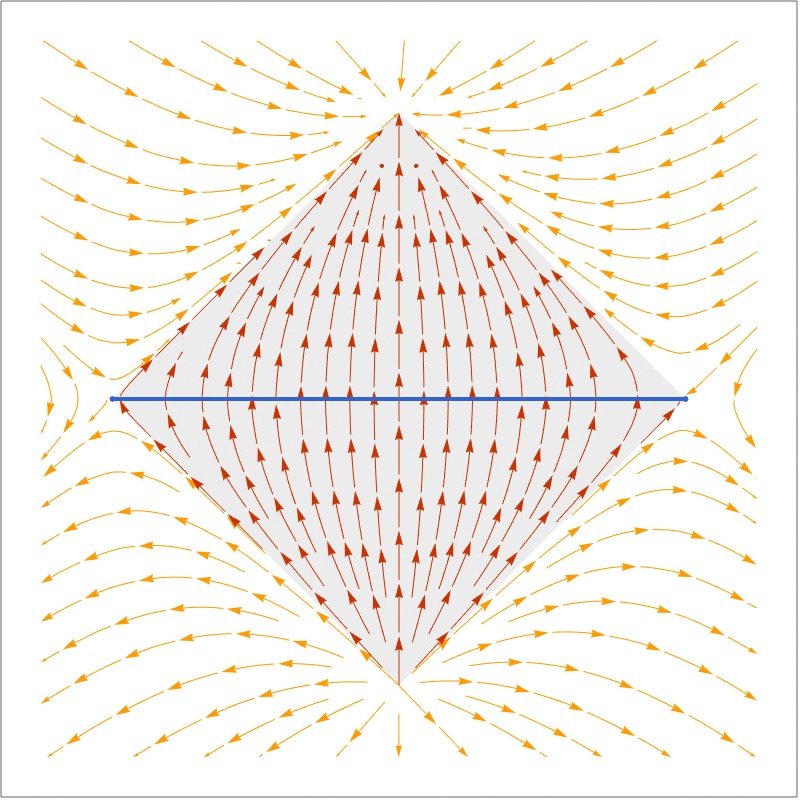
\includegraphics[width=.4\linewidth]{img/modFlowLorentzian.png}
	\hspace{2em}
	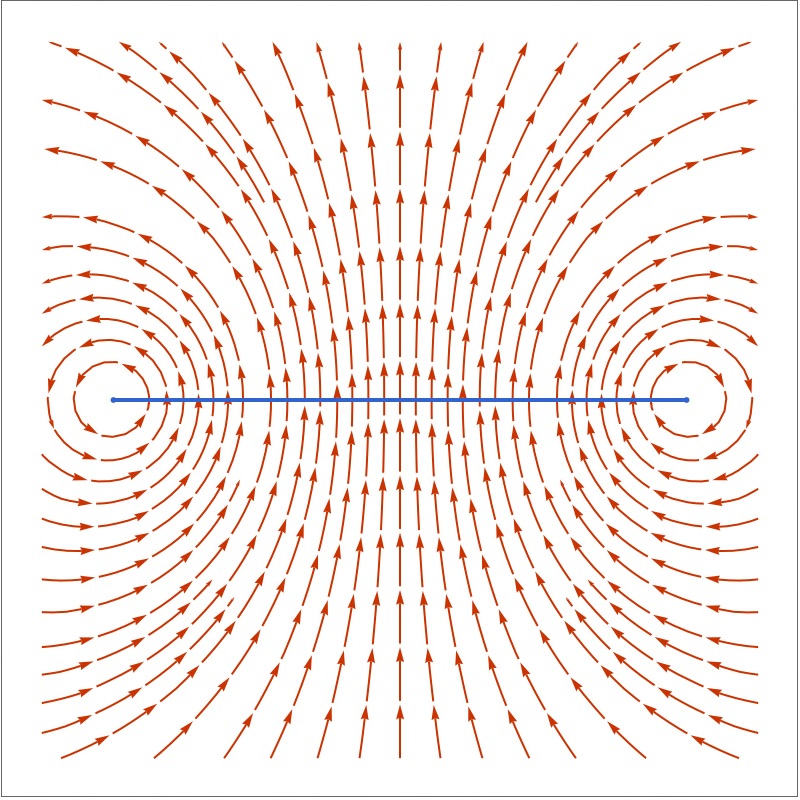
\includegraphics[width=.4\linewidth]{img/modFlowEuclidean.png}
%	\vspace{-2ex}
	\caption{Modular flow at the boundary, for an interval lying on a constant $t = 0$ slice, in Lorentzian and Euclidean signature}
	\end{figure}
	
\pagebreak[4]
	
	We now restrict to an interval centered at the origin: $
		u_\pm v_\pm
		= x^2_\pm - t^2_\pm
		= (\frac{L_\infty}{2})^2
	$, where $x_\pm = -x_\mp$, and same for $t_\pm, u_\pm, v_\pm$. 
	We then introduce the \textit{rapidity} $\theta$ to nicely parametrized the boosted interval; for a constant time slice, we have $\theta = 0$. For a general boosted interval, we have:
	\begin{equation}
		x_\pm = \pm \frac{L_\infty}{2} \cosh \theta,
	\quad
		t_\pm = \pm \frac{L_\infty}{2} \sinh \theta,
	\end{equation}
	For now the coordinates $u_\pm, v_\pm, x_\pm, t_\pm$ and the coordinate length $L_\infty$ are all specified at $z\to 0$, i.e.~at the \textbf{asymptotic boundary}. Note that the RT surface lies on the plane $
		t_\pm / x_\pm = \tanh \theta
	$, namely $\theta$ is constant along the RT surface. 
	We have:
	\begin{gather}
	\begin{aligned}
		\xi &= \frac{2\pi}{L_\infty} \bigg\{
			\pqty\Big{
				\pqty{
					(\tfrac{L_\infty}{2})^2 - z^2
					- (t^2 + x^2)
				} \cosh\theta
				+ 2tx \sinh\theta
			} \,\pdd{t}
		\\ &\qquad\qquad 
			+ \pqty\Big{
				\pqty{
					(\tfrac{L_\infty}{2})^2 - z^2
					+ (t^2 + x^2)
				} \sinh\theta
				- 2tx \cosh\theta
			} \,\pdd{x}
		\\ &\qquad\qquad 
			+ \pqty\big{
				x\sinh\theta
				- t\cosh\theta
			} \,2z\pdd{z}
		\bigg\}
	\end{aligned}
	\end{gather}
	
	We note that the $\pdd{z}$ term vanishes in the following two cases:
	\begin{itemize}[noitemsep,topsep=0pt]
	\item as $z\to 0$, i.e.~near the asymptotic boundary;
	\item within the whole plane: $
			x\sinh\theta
			= t\cosh\theta
		$ where the RT surface lies. 
	\end{itemize}

\FloatBarrier

\pagebreak

%%%%%%%%%%%%%%%%%%%%%%%%%%%%%%%%%%%%%%%%%%%%%%
\bibliographystyle{JHEP} 
\bibliography{cutoffModular-alpha.bib}
%%%%%%%%%%%%%%%%%%%%%%%%%%%%%%%%%%%%%%%%%%%%%%




%%%%%%%%%%%%%%%%%%%%%%%%%%%%%%%%%%%%%%%%%%%%%%
%%%%%%%%%%%%%%%%%%%%%%%%%%%%%%%%%%%%%%%%%%%%%%
%%%%%%%%%%%%%%%%%%%%%%%%%%%%%%%%%%%%%%%%%%%%%%
\end{document}
%%%%%%%%%%%%%%%%%%%%%%%%%%%%%%%%%%%%%%%%%%%%%%
%%%%%%%%%%%%%%%%%%%%%%%%%%%%%%%%%%%%%%%%%%%%%%
%%%%%%%%%%%%%%%%%%%%%%%%%%%%%%%%%%%%%%%%%%%%%%
